\documentclass[10pt,journal,compsoc]{IEEEtran}
\usepackage[obeyspaces]{url}

\usepackage{graphicx}
\usepackage{caption}
\usepackage{float}
\usepackage{subcaption}
\usepackage{hyperref}
\usepackage{cleveref}
\usepackage{listings}

% *** CITATION PACKAGES ***
%
\ifCLASSOPTIONcompsoc
  \usepackage[nocompress]{cite}
\else
  \usepackage{cite}
\fi

% *** GRAPHICS RELATED PACKAGES ***
%
\ifCLASSINFOpdf
\else
\fi

\newcommand\MYhyperrefoptions{bookmarks=true,bookmarksnumbered=true,
pdfpagemode={UseOutlines},plainpages=false,pdfpagelabels=true,
colorlinks=true,linkcolor={black},citecolor={black},urlcolor={black},
pdftitle={DDoS Network Flow Forensics Analyser},%<!CHANGE!
pdfsubject={Big Data project},%<!CHANGE!
pdfauthor={Cristian Turetta, Andrea Perazzoli},%<!CHANGE!
pdfkeywords={Computer Society, DDoS, Forensics, BigData, Data Science, Hadoop, Python}}
             
% correct bad hyphenation here
\hyphenation{op-tical net-works semi-conduc-tor}

\begin{document}
\title{DDoS Network Flow Forensics Analyser}

\author{Cristian~Turetta,~\IEEEmembership{VR421196}
        and~Andrea~Perazzoli,~\IEEEmembership{VR421197}% <-this % stops a space
}

% The paper headers
\markboth{May~2019}%
{Shell \MakeLowercase{\textit{et al.}}:}

\IEEEtitleabstractindextext{
\begin{abstract}
Distributed denial-of-service (DDoS) is a rapidly growing problem. The multitude and variety of both the attacks and the defense approaches is overwhelming. In this report we propose a tool which analyse, using big data framework, recorded traffic and by using statistical tools like standard deviation and difference from mean, it tries to detect the set or at least a subset of attackers using distributed calculus approach, justified by the enormous size of network sniffing records.  We performed experiments with three datasets and our results affirm that the proposed methods can differentiate DoS or DDoS attacks from legitimate traffics.    
\end{abstract}
}

% make the title area
\maketitle

\IEEEdisplaynontitleabstractindextext
\IEEEpeerreviewmaketitle

% sections area
\section{Introduction}
Denial of Service (DoS) attack is launched to make an internet resource unavailable often by overwhelming the victim with a large number of requests. DoS attacks can be categorized on the basis of single source and multi source. Multi source attacks are called distributed Dos or DDoS attacks\cite{ddos_forensics}.
 
There are various type of tool in order to detect and deal with DDoS attacks, these tools can be applied in real time, such as intrusion detection systems (IDS) or by analysing network flow records offline doing a forensics analysis, which is our focus.
Computing forensics analysis over a recorded network flow can be useful, we may understand if someone is trying to flood a network to get a denial of service and eventually recognise it.
Evidence of such intrusions is required in case the affected wants to pursue the court and legal action is to be taken against the adversary.
Forensics investigations are not trivial to accomplish and often done manually, this because the attacker can mask its attempts by mixing legitimate requests with malicious ones.

DDoS attacks aim to compromise the availability of a system or a network, the attack is launched by the adversary which has take control over bots, compromised machines connected to internet, that sends several requests to the victim and overwhelm it with large amount of traffic. This creates a bottleneck and the victim can no further deal with this traffic denying service to them.
During DDoS attacks, the log files swell up to huge sizes, these log files if analysed properly and effectively can help detect and recover from a DDoS attack \cite{ddos_forensics}. Log files can take a long time if processed through conventional means thus we decide to use big data's tool and framework in order to get a faster processing and investigation.

In this report we present our tool which uses \textit{Pig-latin} script embedded into a \textit{Python} program that can be used to analyse network log file, \texttt{pcap} format\cite{wireshrk_pcap}, and returns statistical information about the recorded traffic, since there are a lot of attack variety, we focus on one of the principals which is UDP flood. 
It can be initiated by sending a large number of UDP packets to random ports on a remote host.

This report is structured as follows, in Section 2 we present the statistical tool used in our analysis. In Section 3 we present the project structure and implementation. In Section 4 we focus on analysis results. In Section 5 we discuss the performance of our tool in terms of computational time and resources. Section 6 concludes the report with our considerations.  
\section{Background}
In this section we are introducing the big data framework at the basis of our project, the following paragraphs are useful in order to give a short description and explanation of what we used.  
During project's planning stage, unlike \cite{ddos_forensics} we use \textit{Pig Latin} instead of Java \textit{Map Reduce} because for our purpose it fits better as we are going to understand later on this section. 

\textbf{Apache Pig} is a platform for analysing large datasets. Pig's language, \textit{Pig Latin}, lets you specify a sequence of data transformations such as merging data sets, filtering them, and applying functions to records or groups of records. Pig comes with many built-in functions but you can also create your own user-defined functions to do special-purpose processing.
Pig Latin programs run in a distributed fashion on a cluster, programs are complied into \textbf{Map Reduce} jobs and executed using Hadoop \cite{pig_wiki}.

\textbf{Map Reduce} is a programming model for expressing distributed computations on massive amounts of data and an execution framework for large-scale data processing on clusters of commodity servers. The only feasible approach to tackling large-data problems today is to divide and conquer, the basic idea is to partition a large problem into smaller sub-problems. To the extent that the sub-problems are independent, they can be tackled in parallel by different workers  threads in a processor core, cores in a multi-core processor, multiple processors in a machine, or many machines in a cluster. Intermediate results from each individual worker are then combined to yield the final output.
The general principles behind divide-and-conquer algorithms are broadly applicable to a wide range of problems in many different application domains. One of the most significant advantages of MapReduce is that it provides an abstraction that hides many system-level details from the programmer \cite{jimmy_lin}.

Pig Latin abstracts the programming from the Java MapReduce idiom into a notation which makes MapReduce programming high level, similar to that of SQL for relational database management systems.
\section{Mathematical Models}
\label{sec:mathmodel}
Based on data volume rates, we do need mathematical models to identify which are the source addresses that may be proponents of an attack. 
In letterature we found different approaches, \cite{detection_by_path_analaysis} categorise data into predictable and non predictable data, their mathematical models must be able judge the data by using a threshold. These possible models are the tools for self-similarity analysis such as correlation coefficient and distance matrix. They \cite{detection_by_path_analaysis} use \textit{Pearson's correlation coefficient}, which is defined as:

\begin{equation}
\label{eq:pearson_corr}
	\rho_{X, Y} = \frac{E[(X-\mu_{X})(Y-\mu_{Y})]}{\sigma_X\sigma_Y}
\end{equation}

The correlation is used to measure dependence between two quantities (variables) $X$ and $Y$ with expected values $\mu_X$ and $\mu_Y$ and standard deviations $\sigma_X$ and $\sigma_Y$. Both value of the standard deviations are finite and nonzero ($0 < \sigma_X< \infty$ and $0 < \sigma_Y < \infty$). One of the impressive properties of the correlation is symmetric measurement, in other words, whichever data comes first, we can still get the same result as measuring. In paper \cite{detection_by_path_analaysis} they propose several methodology algorithms, we report two of them
\begin{enumerate}
	\item Correlation between arrival rate and sequence number.
	Denoted $X$ as a sample set of arrival rate ($X = {\label{_k}}$, where $k=$ 0, 1, 2, ..., N) and $Y$ as a sample set of sequence number ($Y = {k}$  where $k=$ 0, 1, 2, ..., N). Calculate the correlation value $(\rho_{X, Y})$ from the two variables: $X$ and $Y$. The expected value is between $-1$ and $1$, $-1 > \rho_{X, Y} > 1 $.
	\item Correlation of self arrival rate. Denoted $X$ as a sample sequence of arrival rate ($X = {\lambda_{(2k)}}$, where $k=$ 0, 1, 2, ..., N) and $Y$ as a sequence number of time interval ($Y = {\lambda_{(2k + 1)}}$ where $k=$ 0, 1, 2, ..., N). Calculate the correlation value $(\rho_{X, Y})$ from the two variables: $X$ and $Y$. The expected value is between $-1$ and $1$, $-1 > \rho_{X, Y} > 1 $.
\end{enumerate}
In order to use the previous mentioned methodology, \cite{detection_by_path_analaysis} define two thresholds: upper $\tau_U$ and lower $\tau_L$. The value of the upper threshold must not exceed 1 and be less than the lower threshold, on the other hand, the value of the lower threshold must not be below 0 and greater than the upper threshold.
These thresholds will help to identify the dependency degree of dependency of the arrival rate data into two categories.
\begin{enumerate}
	\item \textit{Predictable attack rate}: the data will be classified as a predictable attack rate if the correlation value is closed to 0 or 1.
	\item \textit{Nonpredictable attack rate}: the data will be classified as a nonpredictable attack rate if the correlation value is not closed to 0 or 1.
\end{enumerate} 
Unfortunately, only one correlation result $\rho_{X, Y}$ cannot
determine whether arrival data is attacking or legitimate, it is
needed a series of correlation result to confirm the situation.
The attack detection must respond as quickly as possible after the attack reaches the victim by using these methods, doing an online analysis.

Since we categorise data, using big data framework in order to analyse log files offline, which may contains attacks, we can not use methodology proposed by \cite{detection_by_path_analaysis}. Using big data we elaborate the log files in order to extract features used for our analysis. For simplicity we explain each one by referring to a single entry which represents an exchange between a source IP and server.

\begin{itemize}
	\item \textit{n\_packets} \\ Represents the amount of packets.
	\item \textit{total\_volume} \\ It is the sum of all packets length.
	\item \textit{time\_difference} \\ It is the time difference between the first communication and the last one, we consider it as a time window.
	\item \textit{ratio\_vol\_td} \\ Represents the volume over seconds exchanged during the time window.
\end{itemize}

The mathematical model must be able to judge the data by using a thresholds, these ones will be provided by our mathematical tool as we will se further on this sections. Other mathematical model are treated in  \cite{detection_by_path_analaysis} even though we reported the important one. 

Using \textit{python} in order to manipulate the results returned by \textit{Pig} we decide to use \textbf{standard deviation} as graphical guideline model together with the mean and  \textbf{Quantile Range Outliers} method to identify suspicious source address mathematically.
The formula for the sample standard deviation is

\begin{equation}
\label{eq:standard_dev}
	s = \sqrt{\frac{1}{N-1}\sum_{i=1}^N(x_i - \bar{x})^2}
\end{equation}
where $x_1, x_2\ ...\ x_n$ are the samples values, $\bar{x}$ is the mean and $N$ is the number of samples in the dataset generated by \textit{Pig-latin} script.

The \textit{standard deviation} is a description of the data's spread, how widely it is distributed about the mean.  
A smaller standard deviation indicates that more of the data is clustered about the mean.  
A larger one indicates the data are more spread out.
Using this information, we started to make inferences about the data.  
For example, we could determine whether a particular point was significantly higher above data volume than all others,  whether it represented a statistical anomaly that was worth investigating, based on how many standard deviations away from the mean it was located.

The \textit{quantile range outliers} method of outlier detection uses the quantile distribution of the values in a column to locate the extreme values. Quantiles are useful for detecting outliers because there is no distributional assumption associated with them. Data are simply sorted from smallest to largest. For example, the $20^{th}$ quantile is the value at which 20\% of values are smaller. Extreme values are found using a multiplier of the interquantile range, the distance between two specified quantiles.
In statistics and probability \textit{quantiles} are cut points dividing the range of a probability distribution into continuous intervals with equal probabilities, or dividing the observations in a sample in the same way. 

In our work we decide to identify outliers calculating the $25^{th}$ and the $75^{th}$ percentile then we calculate the interquantile rage by doing $Q_{75}-Q_{25}$. We chose $1.5$ as multiplicative $\alpha$ factor for the interquantile. 
We use this coefficient as \textit{cut off} for determine upper and lower bound for outliers data, these will represent our thresholds. 
The following listing report the code which implements this feature\footnote{In Lst. \ref{lst:qrom} we report only the method applied to data volume exchanged, we do the same for traffic volume (Kb/s)} .
 
 \begin{lstlisting}[numbers=left, columns=flexible, breaklines=true, frame=tb, caption={quantile range outliers method}, label={lst:qrom}]
    q25, q75 = percentile(dataframe['total_volume'], 25), percentile(dataframe['total_volume'], 75)
    inter_quartile_range = q75 - q25
    # calculate the outlier cutoff
    cut_off = inter_quartile_range * 1.5
    lower, upper = q25 - cut_off, q75 + cut_off
    # identify outliers
    data_outliers = [x for x in dataframe['total_volume'] if x < lower or x > upper]
\end{lstlisting}

We decide to output two plots and one file, \textit{data analysis} which figure out the amount of data, in terms of megabyte, exchanged between a source and the server. \textit{Volume analysis} is like the previous one but represents the data volumes per second exchanged between a source and the server. In the \texttt{.txt} file we report the outliers by IP address and values of analysis we calculates, such as traffic volume and data exchanged.
\bigskip

\begin{figure}[ht]
  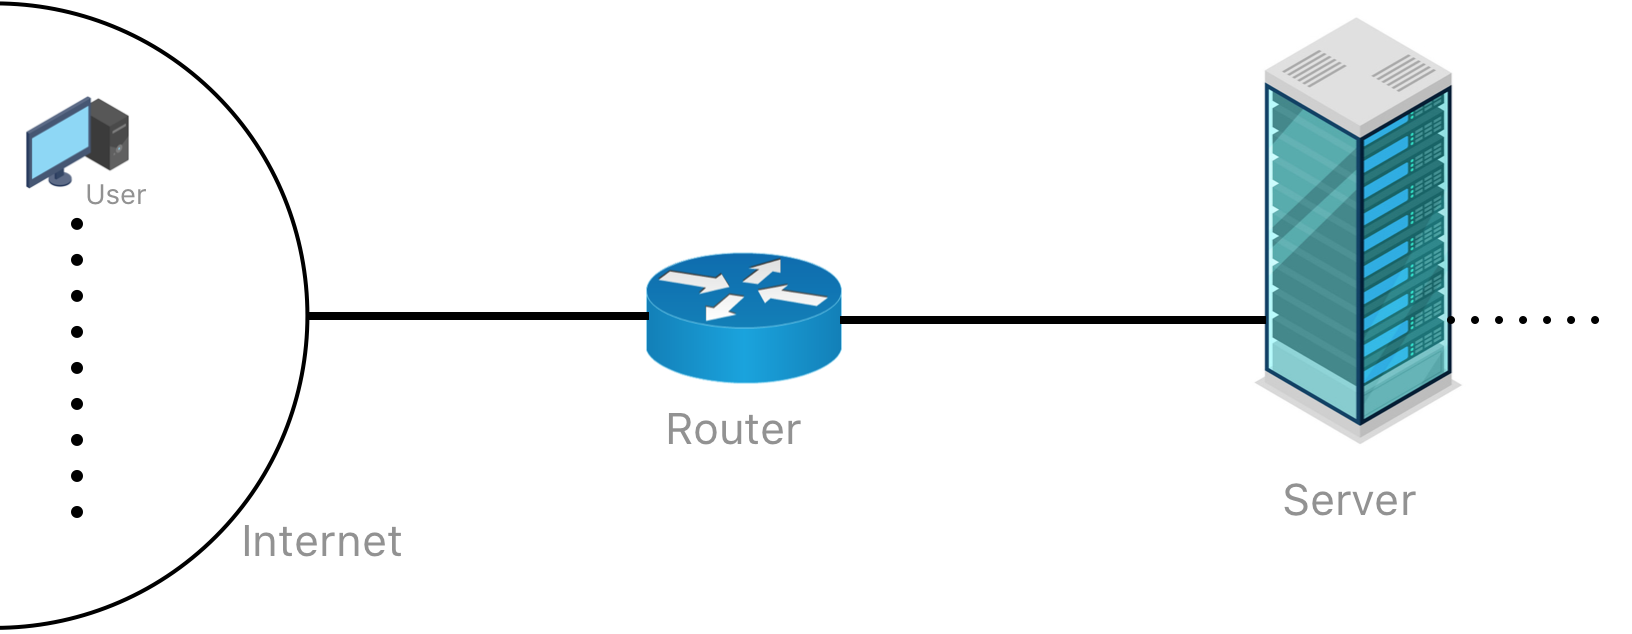
\includegraphics[scale=0.31]{imgs/scenario.png}
  \caption{Network Scenario}
  \label{fig:networkscenario}
\end{figure}

\begin{figure*}[h]
	\begin{subfigure}{0.48\textwidth}
		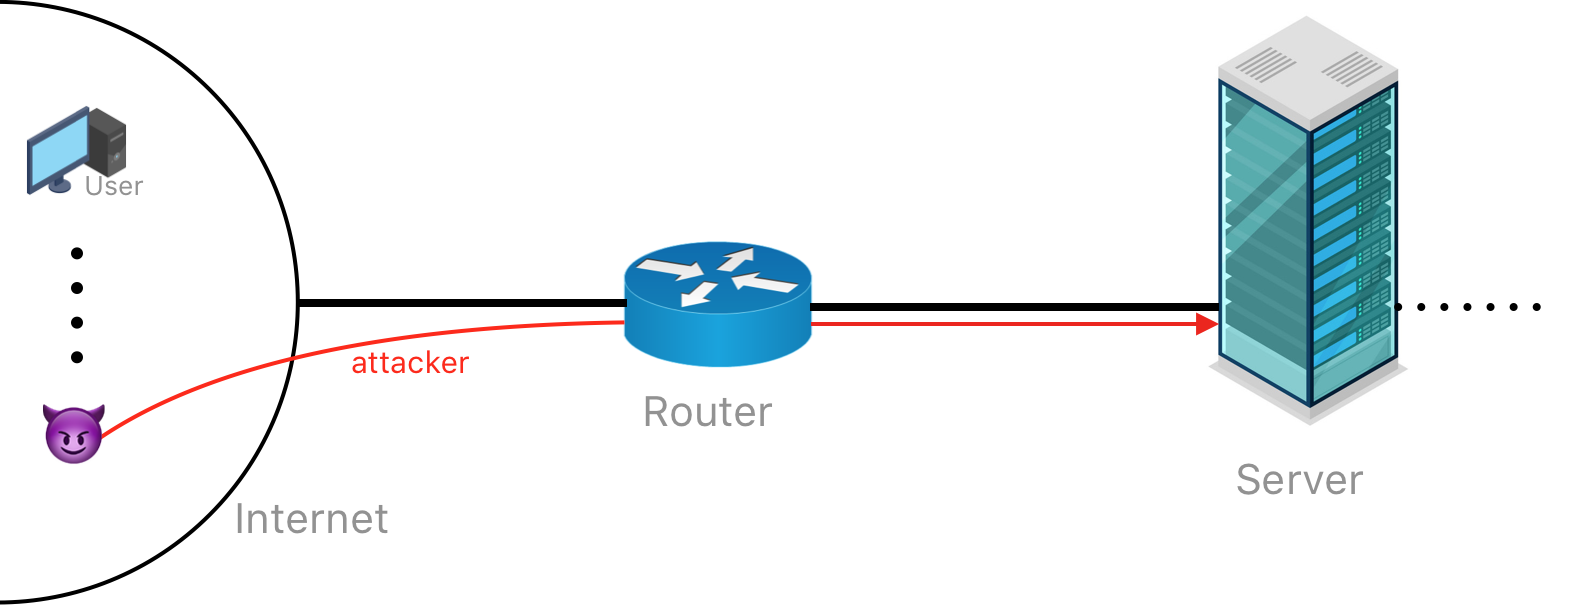
\includegraphics[width=\textwidth]{imgs/DoS_attack.png}
		\caption{DoS attack scenario} \label{fig:DoS}
	\end{subfigure}
	\hspace*{\fill} % separation between the subfigures
	\begin{subfigure}{0.48\textwidth}
		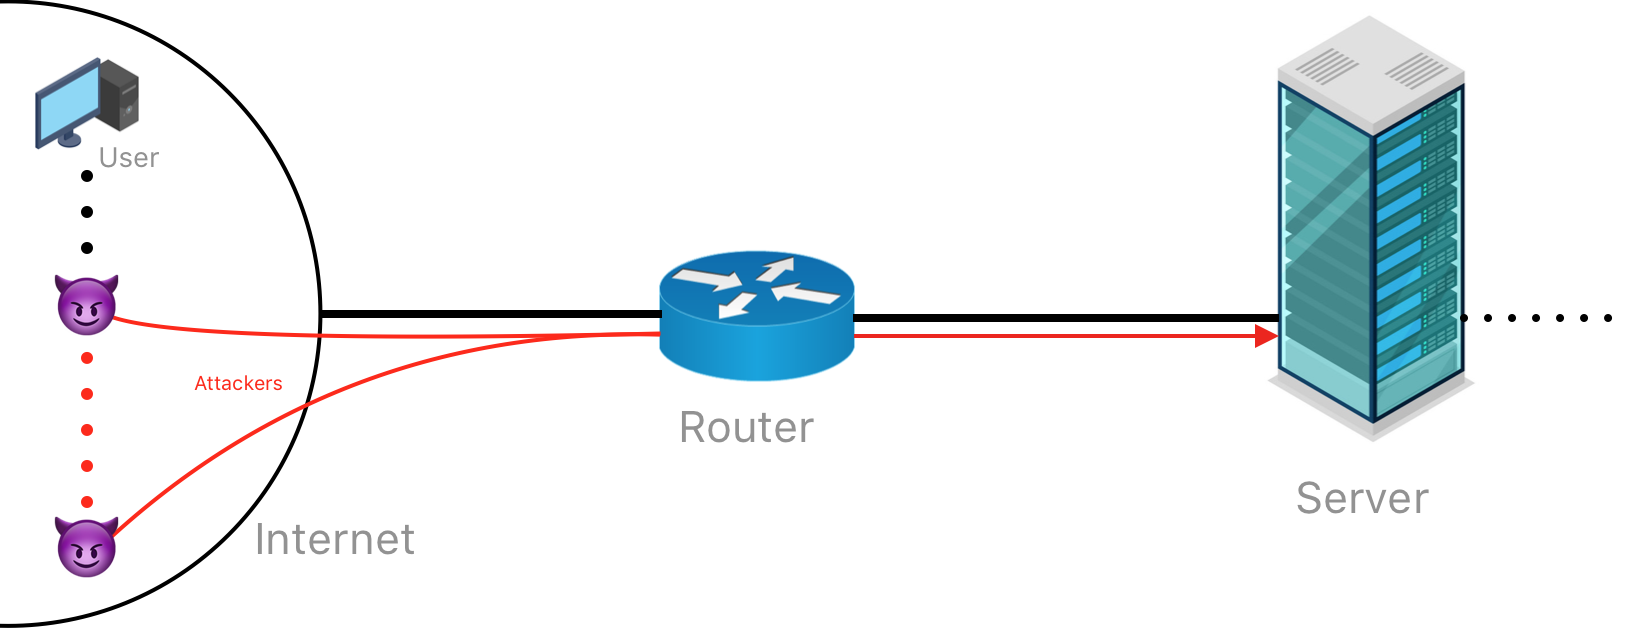
\includegraphics[width=\textwidth]{imgs/DDoS_attack.png}
		\caption{DDoS attack scenario} \label{fig:DDoS}
	\end{subfigure}
	\caption{Attacks scenarios}
	\label{fig:atks}
\end{figure*}

\section{Project structure and implementation}
\label{sec:projstruct}
Our project \cite{proj_repo} and its source code is freely downloadable on \href{https://github.com/CristianTuretta/DDoS-Network-Flow-Forensics-Analyser-.git}{Github}. Here, we focused on the UDP flood D(D)oS analysis of \texttt{.pcap} records: the goal is to point out good and evil users given a \texttt{.pcap} network sniff file converted to \texttt{.csv} format. The project is a multi-layered tool which primarily consists in two executable Python 3 scripts:

\subsection{DDoSAnalysis}
\textit{DDoSAnalysis.py} can be used in two different modes, depending on the line parameters used: 
	\begin{itemize}
		\item \textit{-g dataset\_name n\_members n\_lines n\_attackers atk\_volume atk\_duration} \\Generates a random, bogus dataset in the current working directory with the name specified in the second argument, alongside with the number of normal network users specified in \textit{n\_members} argument, the dimension of the dataset (in lines), the number of infected machines, the attack volume (per packet) and its duration. At the end of the generation process, it copies the dataset into the Hadoop File System. We assumed that Hadoop is installed and a folder tree under \path{hdfs://user/your_user/project/input} exists.
		\item \textit{-a dataset\_name} \\ Begin the analysis of the dataset \textit{dataset\_name} using a Pig script. In order to work, the dataset must have been previously copied into the Hadoop input folder, which automatically happens if the dataset is generated using \textit{-g} option. It saves the elaborated dataset under \path{outputs/dataset_name} with an image consisting of a plot of every agent average velocity (Mbps), an attack volume graph and a statistical image which shows the squared margin to mean velocity.
		\item \textit{-anp dataset\_name} \\ It's like the \textit{-a} argument, but it doesn't start Pig analysis. It's used when we have already completed a Pig analysis, and we only want to aggregate data and obtain the plots. 
		\item \textit{-ga dataset\_name n\_members n\_lines n\_attackers atk\_volume atk\_duration} \\ Launches both the generation and the analysis
		\item \textit{-sga dataset\_name n\_members n\_lines n\_attackers atk\_volume atk\_duration} \\ Launches both the generation and the analysis. After generation but before the Pig analysis, it prints an estimation of the dataset dimension, letting the user choose whether to proceed or not.
	\end{itemize}
The script also automatically records infos about performance timing under \path{PerformanceHistory.csv}.

\subsection{PerformanceAnalyser}
\textit{PerformanceAnalyser.py} is used to automatically plot all the infos stored under \path{PerformanceHistory.csv}. It supports two modes:
	\begin{itemize}
		\item \textit{-a img\_name} \\ Stores a plot under the current working directory named \textit{img\_name} of analysis statistics (history of dataset analyzed and time elapsed)
		\item \textit{-g img\_name} \\ Stores a plot under the current working directory named \textit{img\_name} of dataset generation statistics (history of dataset generated and time elapsed)
	\end{itemize}

\textit{PerformanceAnalyser.py} also exposes a method used as a wrapper to call the generation and analysis routines, using a \textbf{CProfile} python module to gain time statistics.

\bigskip
The first two mentioned scripts are the user interface of our tool. However, we have other core scripts which make the generation/analysis possible:

\subsection{DatasetGenerator}
\textit{DatasetGenerator.py} contains the core generation routine of datasets. It generates a pool of innocent IPs and an attackers' one, then it fills line-by-line the dataset with random and bogus informations, extracting random users and attackers. It saves a csv file in the format: \textit{id, time, source\_ip, dest\_ip, protocol, packet\_size, payload}

\subsection{Evaluator} 
\textit{Evaluator.py} exposes the main routine which processes the Pig script output. It computes the mean velocity of all users, and then produces a plot consisting of the velocity of every single user, represented with a blue line, previously calculated by the Pig script (\textit{udpfloodpcap.pig}) and the mean velocity of all users, represented with a red line. The data scientist could distinguish between evil and good users just looking at the deviation from the average. It also plots a volume comparison graph between users and data margin to mean.

\subsection{Pig script}
\textit{Udpfloodpcap.pig} calculates the mean velocity of every machine given a dataset in input. 
This is the core of the analysis tool: it uses Pig Latin mapreduce paradigm. 
The script loads the dataset, filter the records having UDP protocol, and group them by \textit{(source\_ip, destination\_ip)} tuple. 
At this point we have to handle a list of \textit{map(tuple, bag)} containing all the corresponding packets sent by a machine. 
We can then calculate the number of packets (counting the elements in the bag), the total volume exchanged by a particular machine (summing up the corresponding data for each element of the bag) and the mean velocity in bps (using the total volume divided by the max time minus the min time). 
This is a crucial factor which we use to discriminate good and evil users. Here below some part of code we wrote for prepare the dataset in order to detect UDP flood attack:


\begin{lstlisting}[numbers=right, columns=flexible, breaklines=true, frame=tb, caption={\textit{Udpfloodpcap.pig} script}, label={lst:udpfloodscript}]
udpdataset = FILTER dataset BY protocol == 'UDP';
udpgroup = GROUP udpdataset BY (sourceip, destip);

udpmap = FOREACH udpgroup GENERATE group, ordereddataset.(pkt_n,time,dim), MIN(ordereddataset.time) AS min_ts, MAX(ordereddataset.time) AS max_ts, COUNT(ordereddataset.pkt_n) AS n_packets, SUM(ordereddataset.dim) AS total_volume;

result = FOREACH udpmap GENERATE group, min_ts, max_ts, n_packets,total_volume, (float)(max_ts-min_ts) AS time_difference, (float)(total_volume/(max_ts-min_ts)) AS ratio_vol_td;

\end{lstlisting}

The first line filter the loaded dataset in order to have only UDP packets while the second line group the filtered dataset by source IP and destination IP. 
It is using in line four in order to find for each pair of source and destination IP the following features: timestamp of the first and the last packet exchanged, the number of packets exchanged and the total volume of data exchanged obtained by sum over the packet length feature. 
In line six we calculate an approximated time window of communication between source and destination address and the average speed by dividing the total amount of data exchanged over the time window.
At this point we have highlighted all the necessary features to accomplish our analysis by applying our mathematical model previously illustrated.










   

\begin{figure}[ht]
  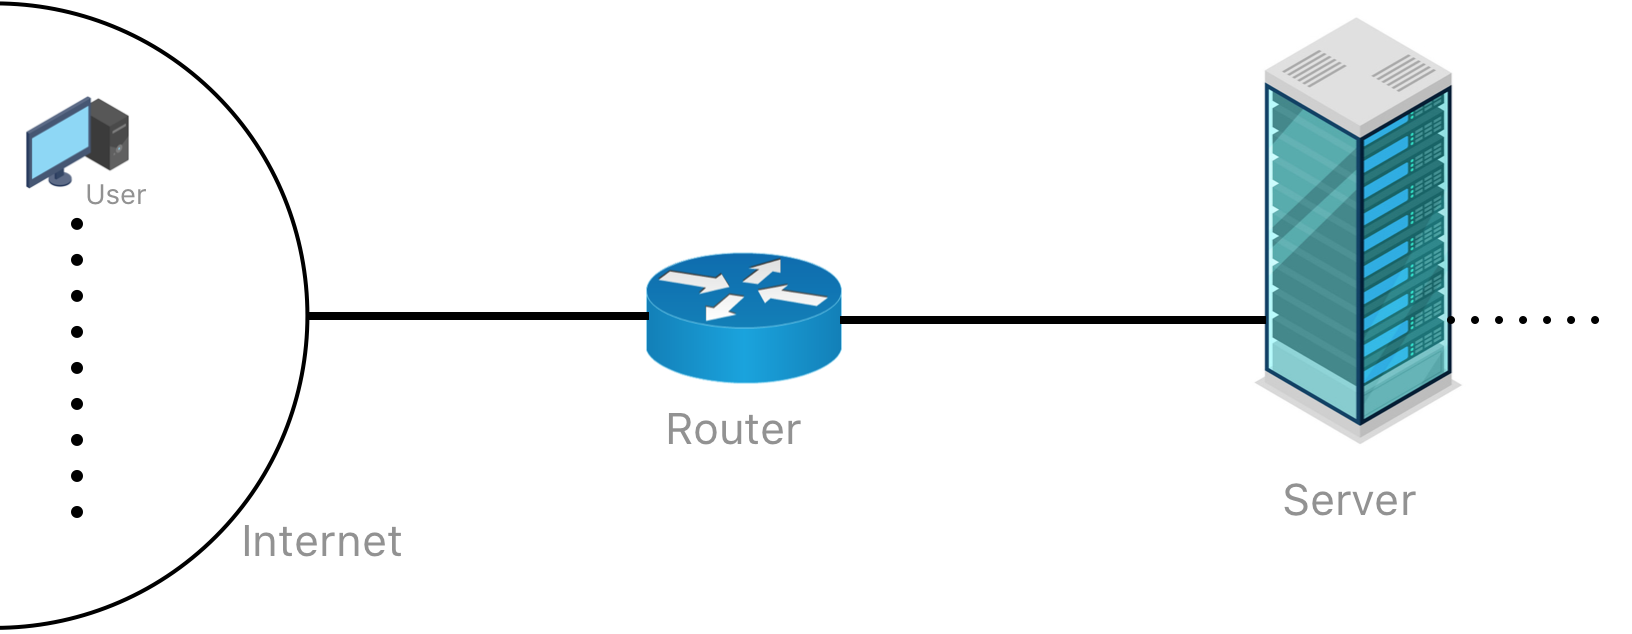
\includegraphics[scale=0.31]{imgs/scenario.png}
  \caption{Network Scenario}
  \label{fig:networkscenario}
\end{figure}

\begin{figure*}[h]
	\begin{subfigure}{0.48\textwidth}
		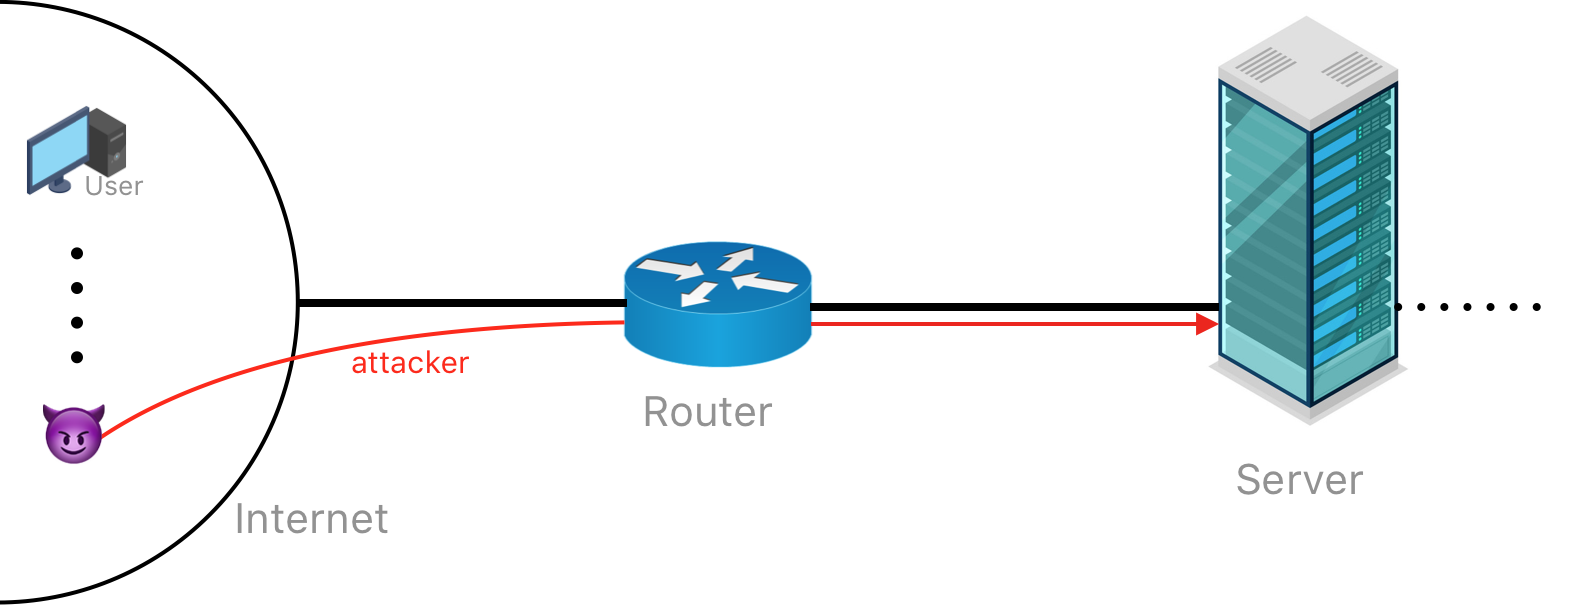
\includegraphics[width=\textwidth]{imgs/DoS_attack.png}
		\caption{DoS attack scenario} \label{fig:DoS}
	\end{subfigure}
	\hspace*{\fill} % separation between the subfigures
	\begin{subfigure}{0.48\textwidth}
		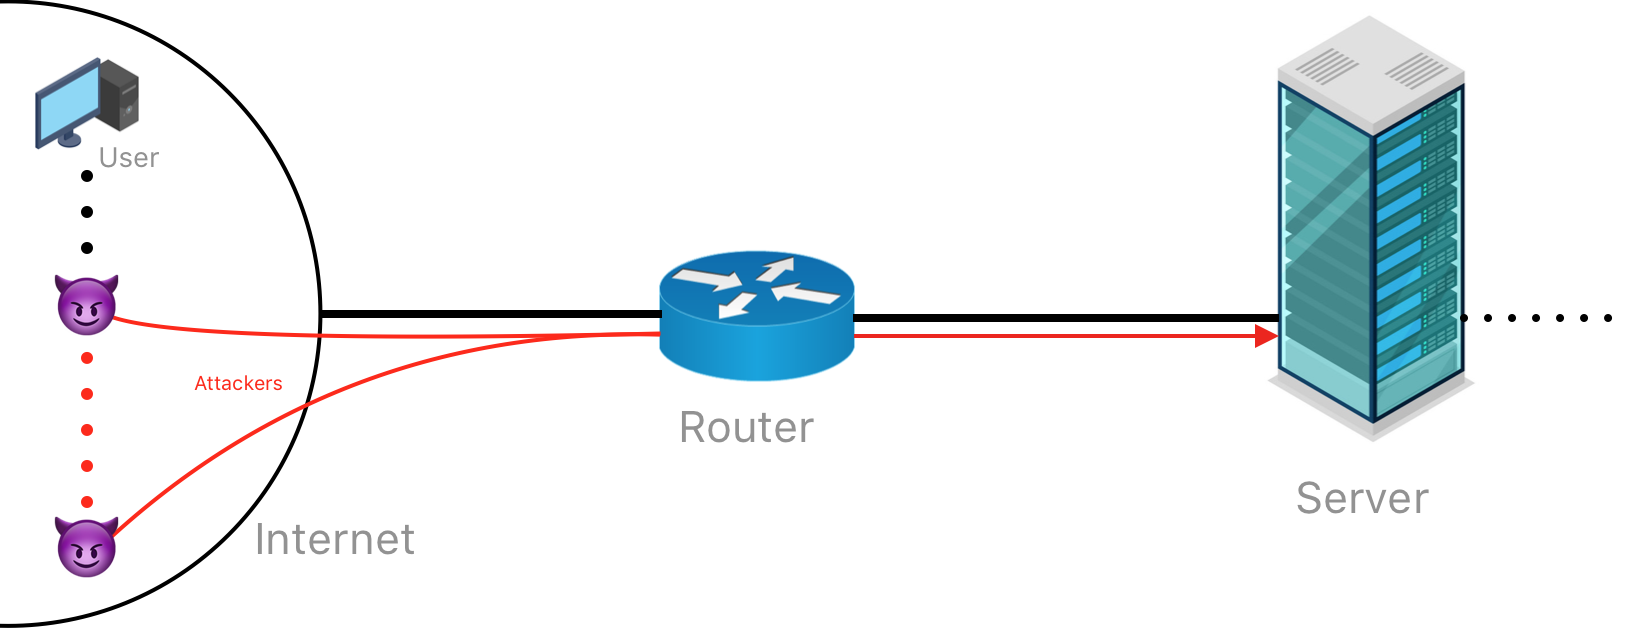
\includegraphics[width=\textwidth]{imgs/DDoS_attack.png}
		\caption{DDoS attack scanrio} \label{fig:DDoS}
	\end{subfigure}
	\caption{Attacks scenarios}
	\label{fig:atks}
\end{figure*}

\section{Analysis}
In this section we will illustrate the scenario on which we have based our analysis and then we will show two examples of attack, DDoS and DoS, in order to explain and evaluate our analysis quality trying to base our conclusion by using different datasets\footnote{Mentioned dataset were generated by our tool, it is possible to analyse every type of dataset on your own if in \texttt{pcap} format.}. There is also a summary of how to configure and run an analysis with \textit{Python} and \textit{Hadoop}.

\subsection{Senario} 
The scenario we focusing on is illustrated in fig.\ref{fig:networkscenario}, as we can see it is a very simple and basic design scenario. There is a \textit{router} that communicates with \textit{internet},  it connects the \textit{sever} with the global network, as we will see further on the treatment \textit{internet} may contains one or several attackers which aim is to deny the service give by the \textit{server}. 

% TODO write here avg stats of server with no attacks.

We choose this type of network configuration in order to concentrate our heed on the implementation of analysis tools and big data scripting, which are the main topics of this project.
 
\subsection{Configuring and Running Analysis}
This tool has been developed for running analysis over network flow records with minimal effort from the user. Once installed and configured \textit{Hadoop} on your PC or cluster, only one line of code is needed for running and storing the results of an analysis, as shown in the example below

\begin{lstlisting}[firstline=1, lastline=1]
   python3 DDoSAnalysis.py -a dataset_name
	Write('Case insensitive '); 
	WritE('Bash keywords.')
\end{lstlisting}

\subsection{DoS Analysis Example}

\subsection{DDoS Analysis Example}





















\begin{figure*}[h]
	\begin{subfigure}{0.48\textwidth}
		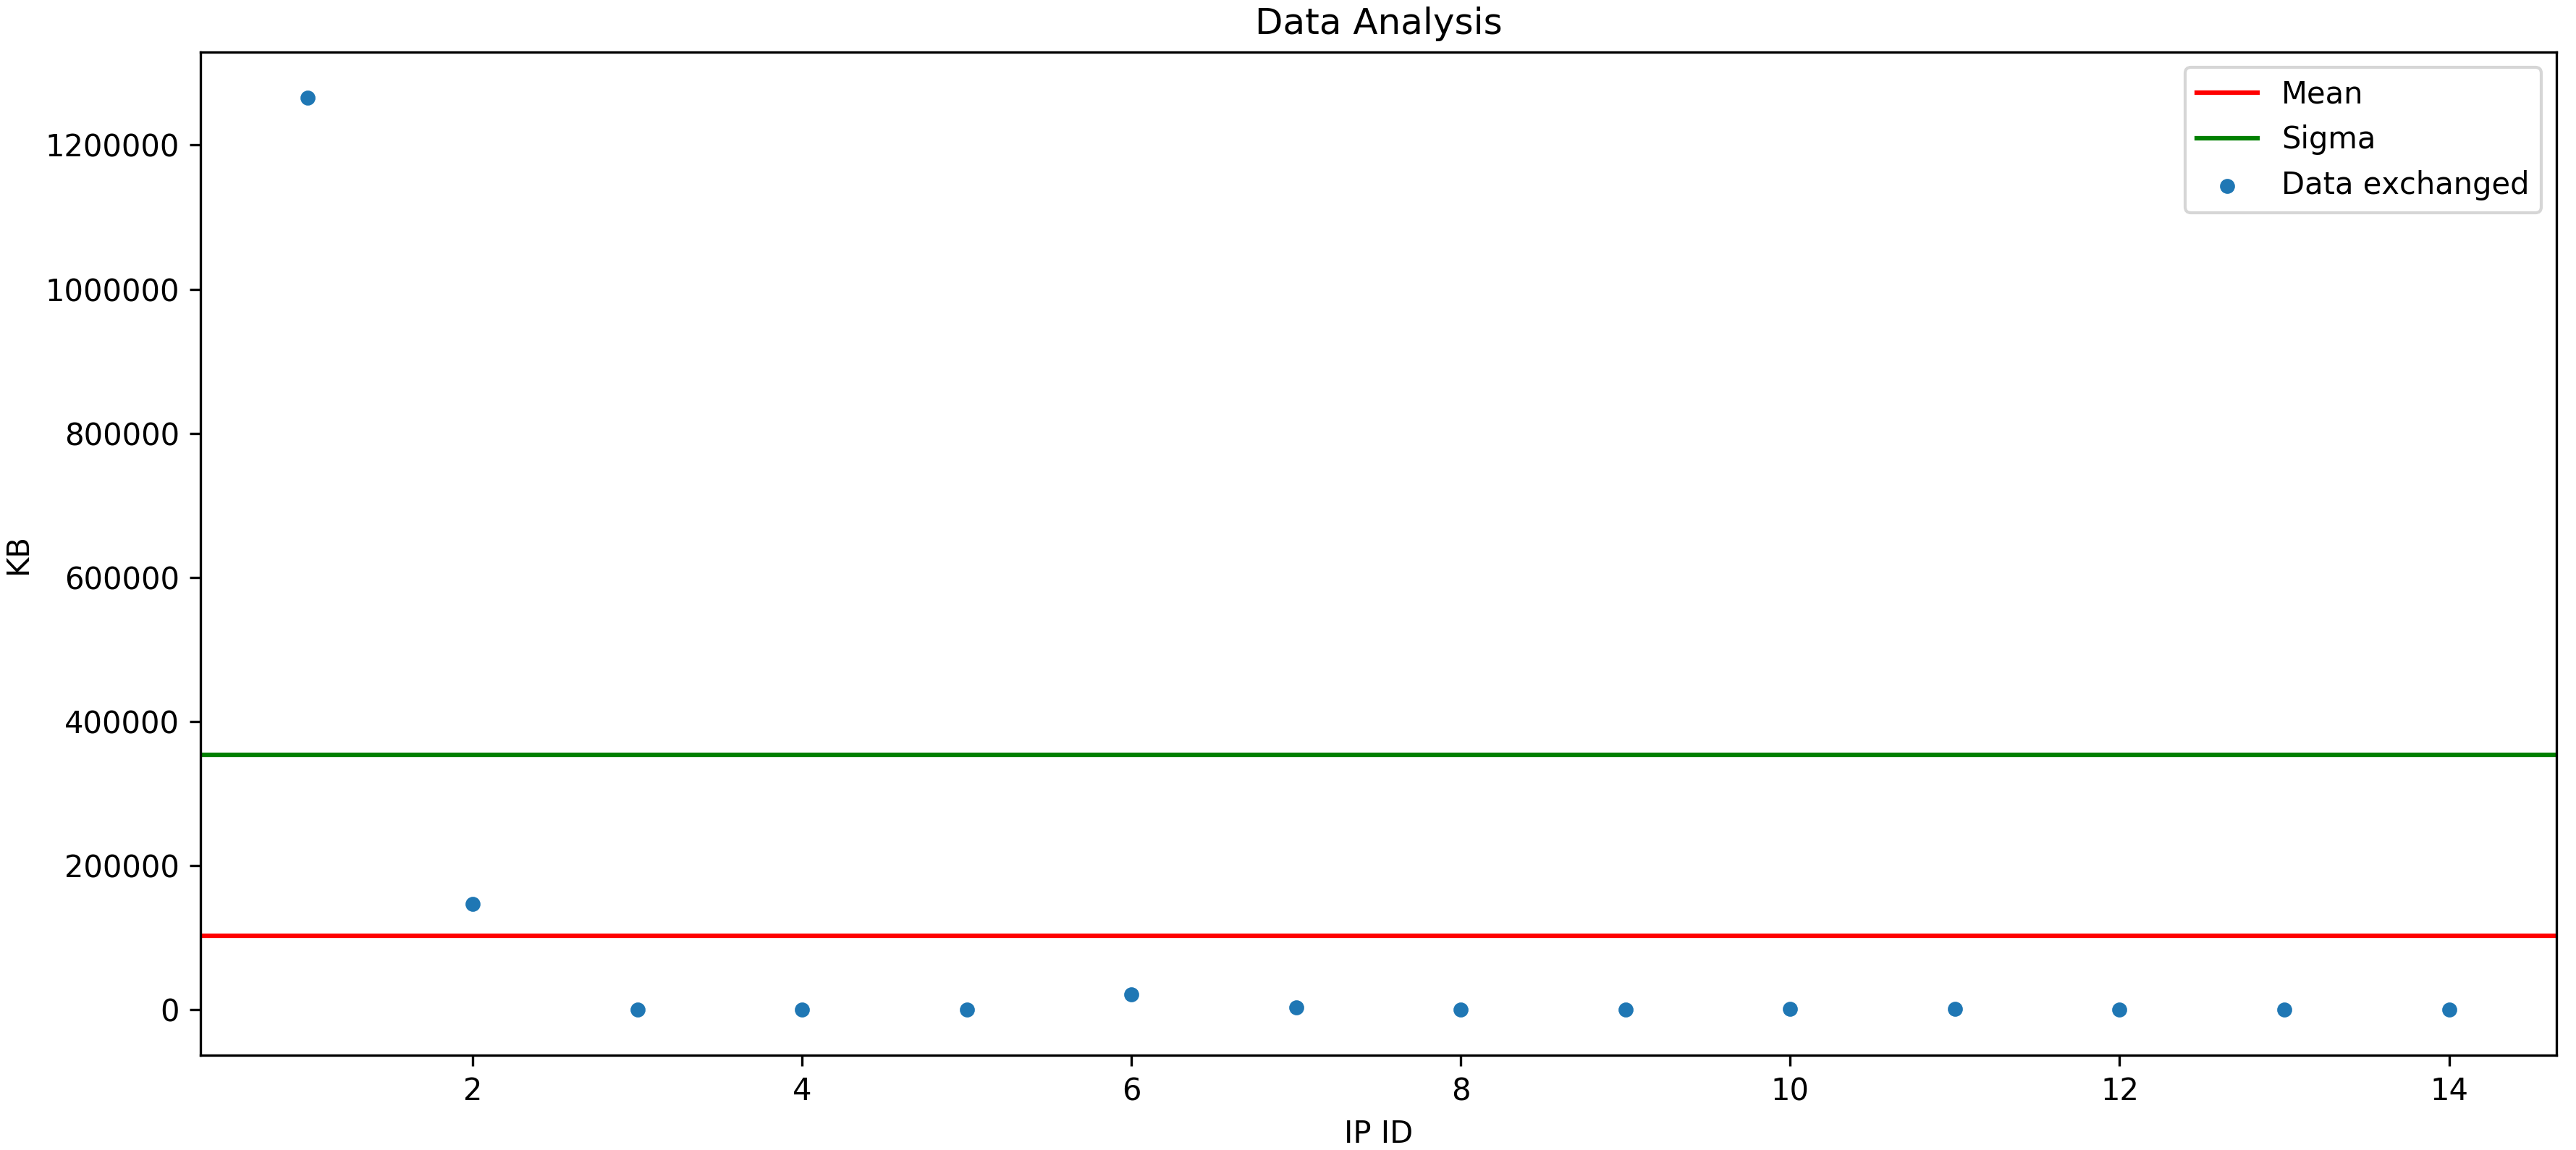
\includegraphics[width=\textwidth]{imgs/DDoSMixed-data_analysis}
		\caption{DDoS Data Analysis} 
		\label{fig:ddos_data}
	\end{subfigure}
	\hspace*{\fill} % separation between the subfigures
	\begin{subfigure}{0.48\textwidth}
		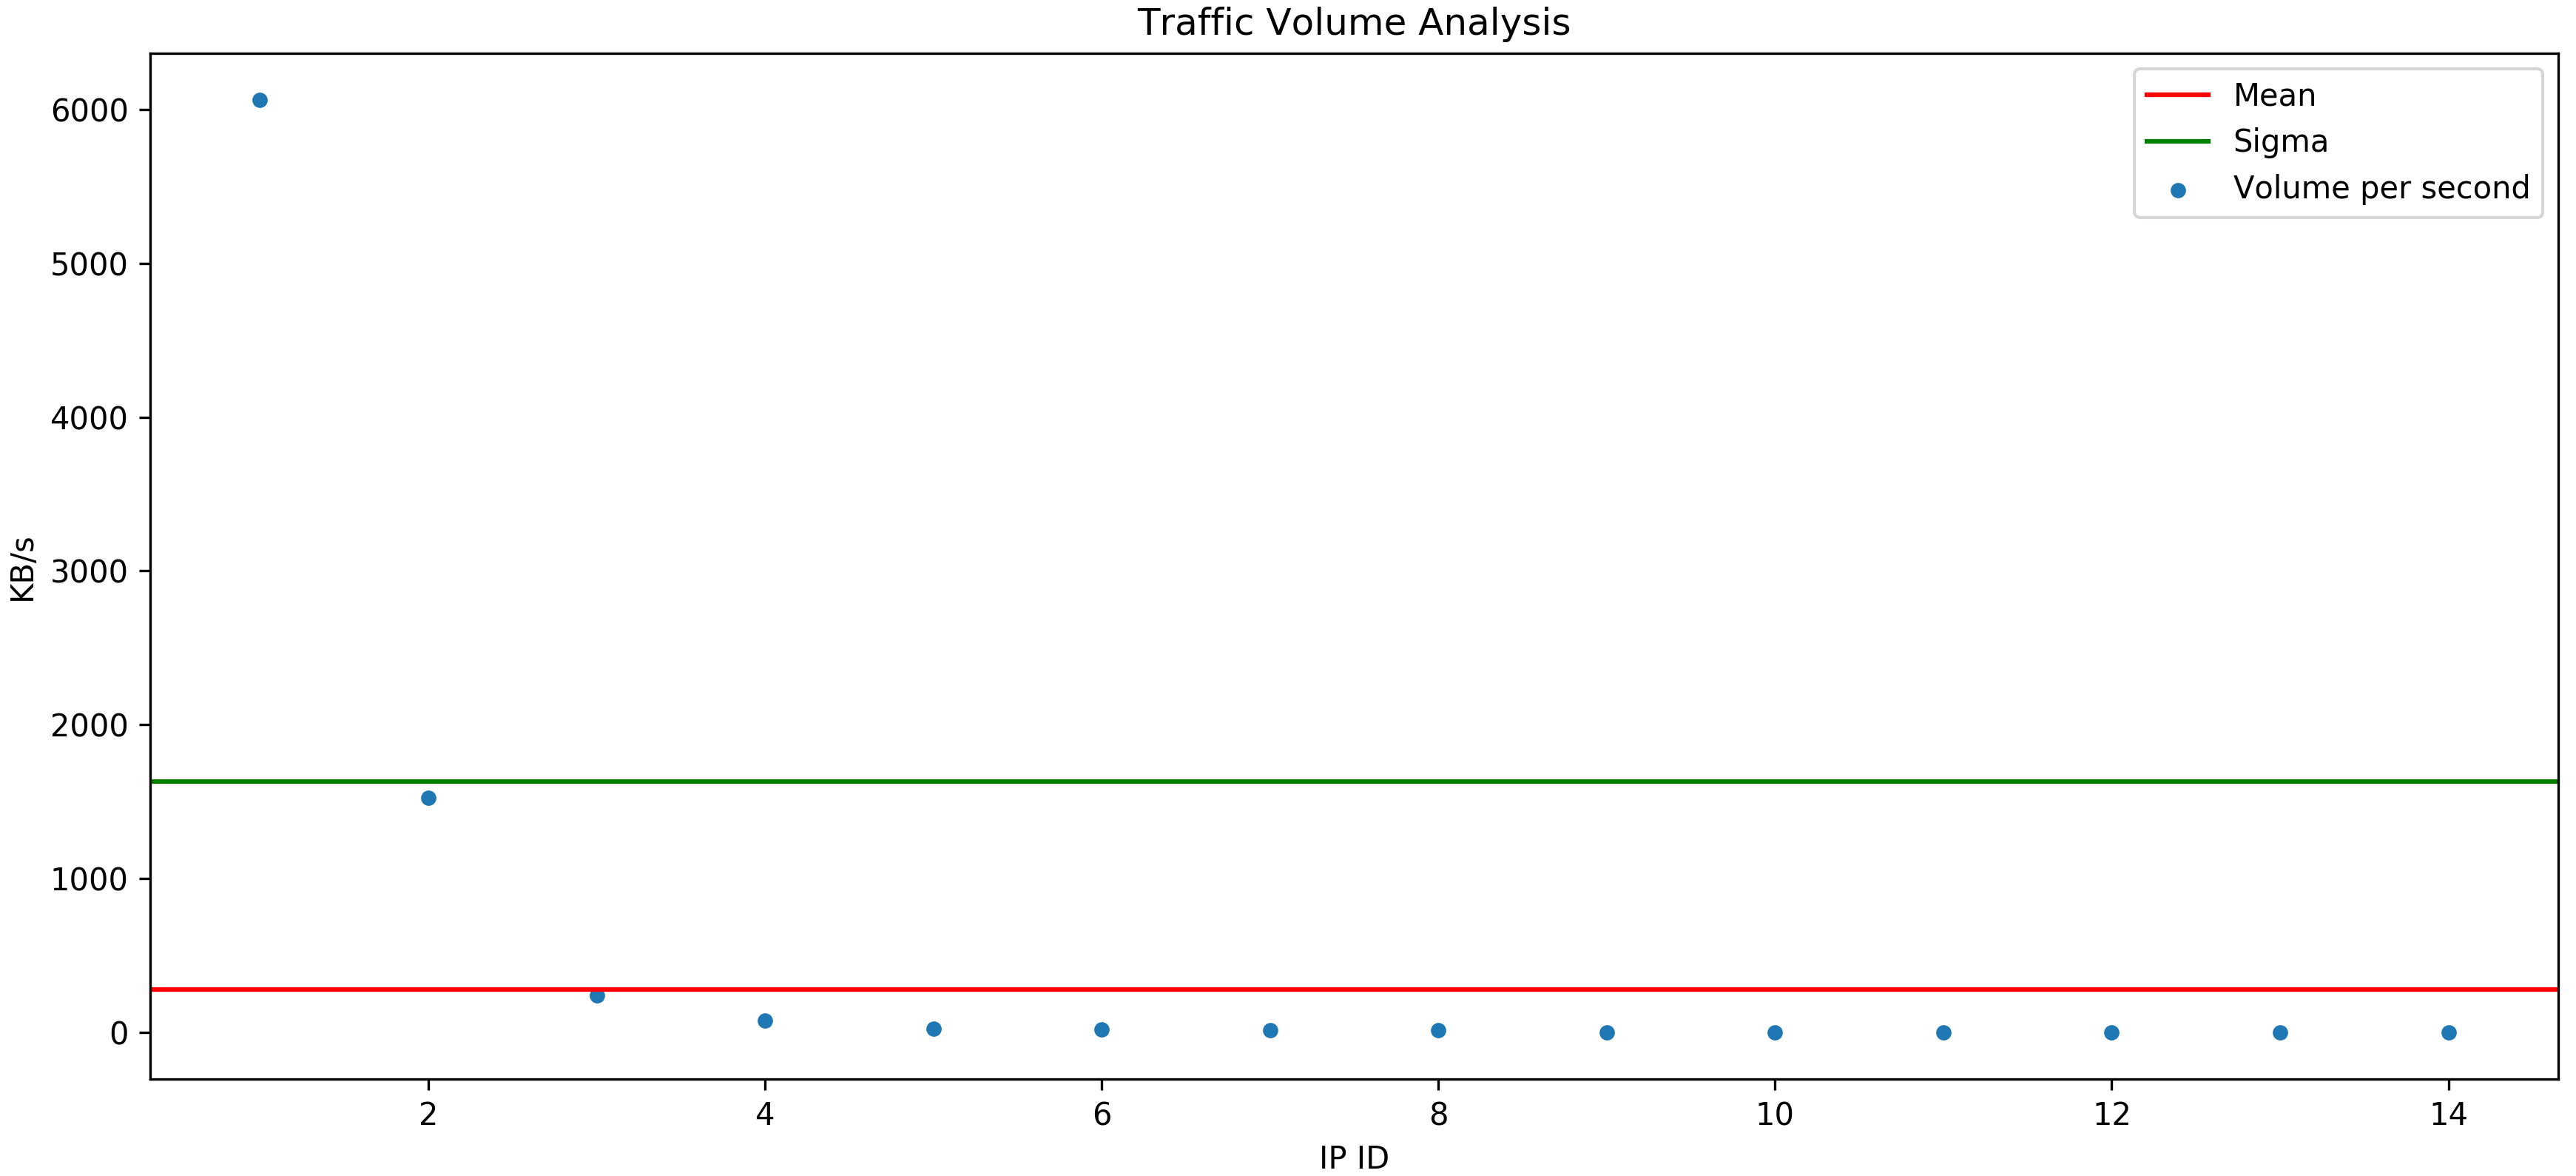
\includegraphics[width=\textwidth]{imgs/DDoSMixed-volume_analysis}
		\caption{DDoS Volume Analysis} 
		\label{fig:ddos_volume}
	\end{subfigure}
	\caption{DDoS attack Analysis}
	\label{fig:ddos_analysis}
\end{figure*}

\section{Performance Analysis}
\label{sec:perfanalysis}
%In our tool we have developer a \textit{script} which records timestamps and duration time of big data analysis in a \texttt{.csv} file, called \texttt{PerformanceHistory.csv}. The \textit{script} mentioned before is used in order to figure out the time of analysis. 
The environment in which we tested our tool is a cluster of the University of Verona, running Ubuntu 18.04.1 LTS, it has an Intel Xeon Processor Skylake (4 cores @ 2,6 GHz) and a RAM memory of 7880 MiB for a single node, in its total configuration it has ten VCore and 60GB of RAM memory. 
We have never observed a total usage of more of 10\% CPU using \texttt{top} command and, in general, memory usage is often below 3000 MiB.
%% TODO DONE performance scritte bene guardando pagina del cluster 
%Using our script called \texttt{PerformanceAnalysis.py} we managed to plot the time elapsed to generate and analyze the datasets listed into Tab. \ref{tab:dataset_info}: results are reported into Fig. \ref{fig:datasets_statistics}.
%We can immediately see that the generation time is much greater for attack datasets: this is justifiable because of the greater size, considering multi-user disk accesses.
%Talking about analysis statistics, we can see a spike in \textit{ddos\_atk} and \textit{no\_atk} datasets. Here, long cluster timeouts during Pig Latin script execution play a great role, and we cannot have much control over it. Without that problem, analysis of the datasets would have taken much less time.
%
%\begin{figure}[ht]
%	\centering
%	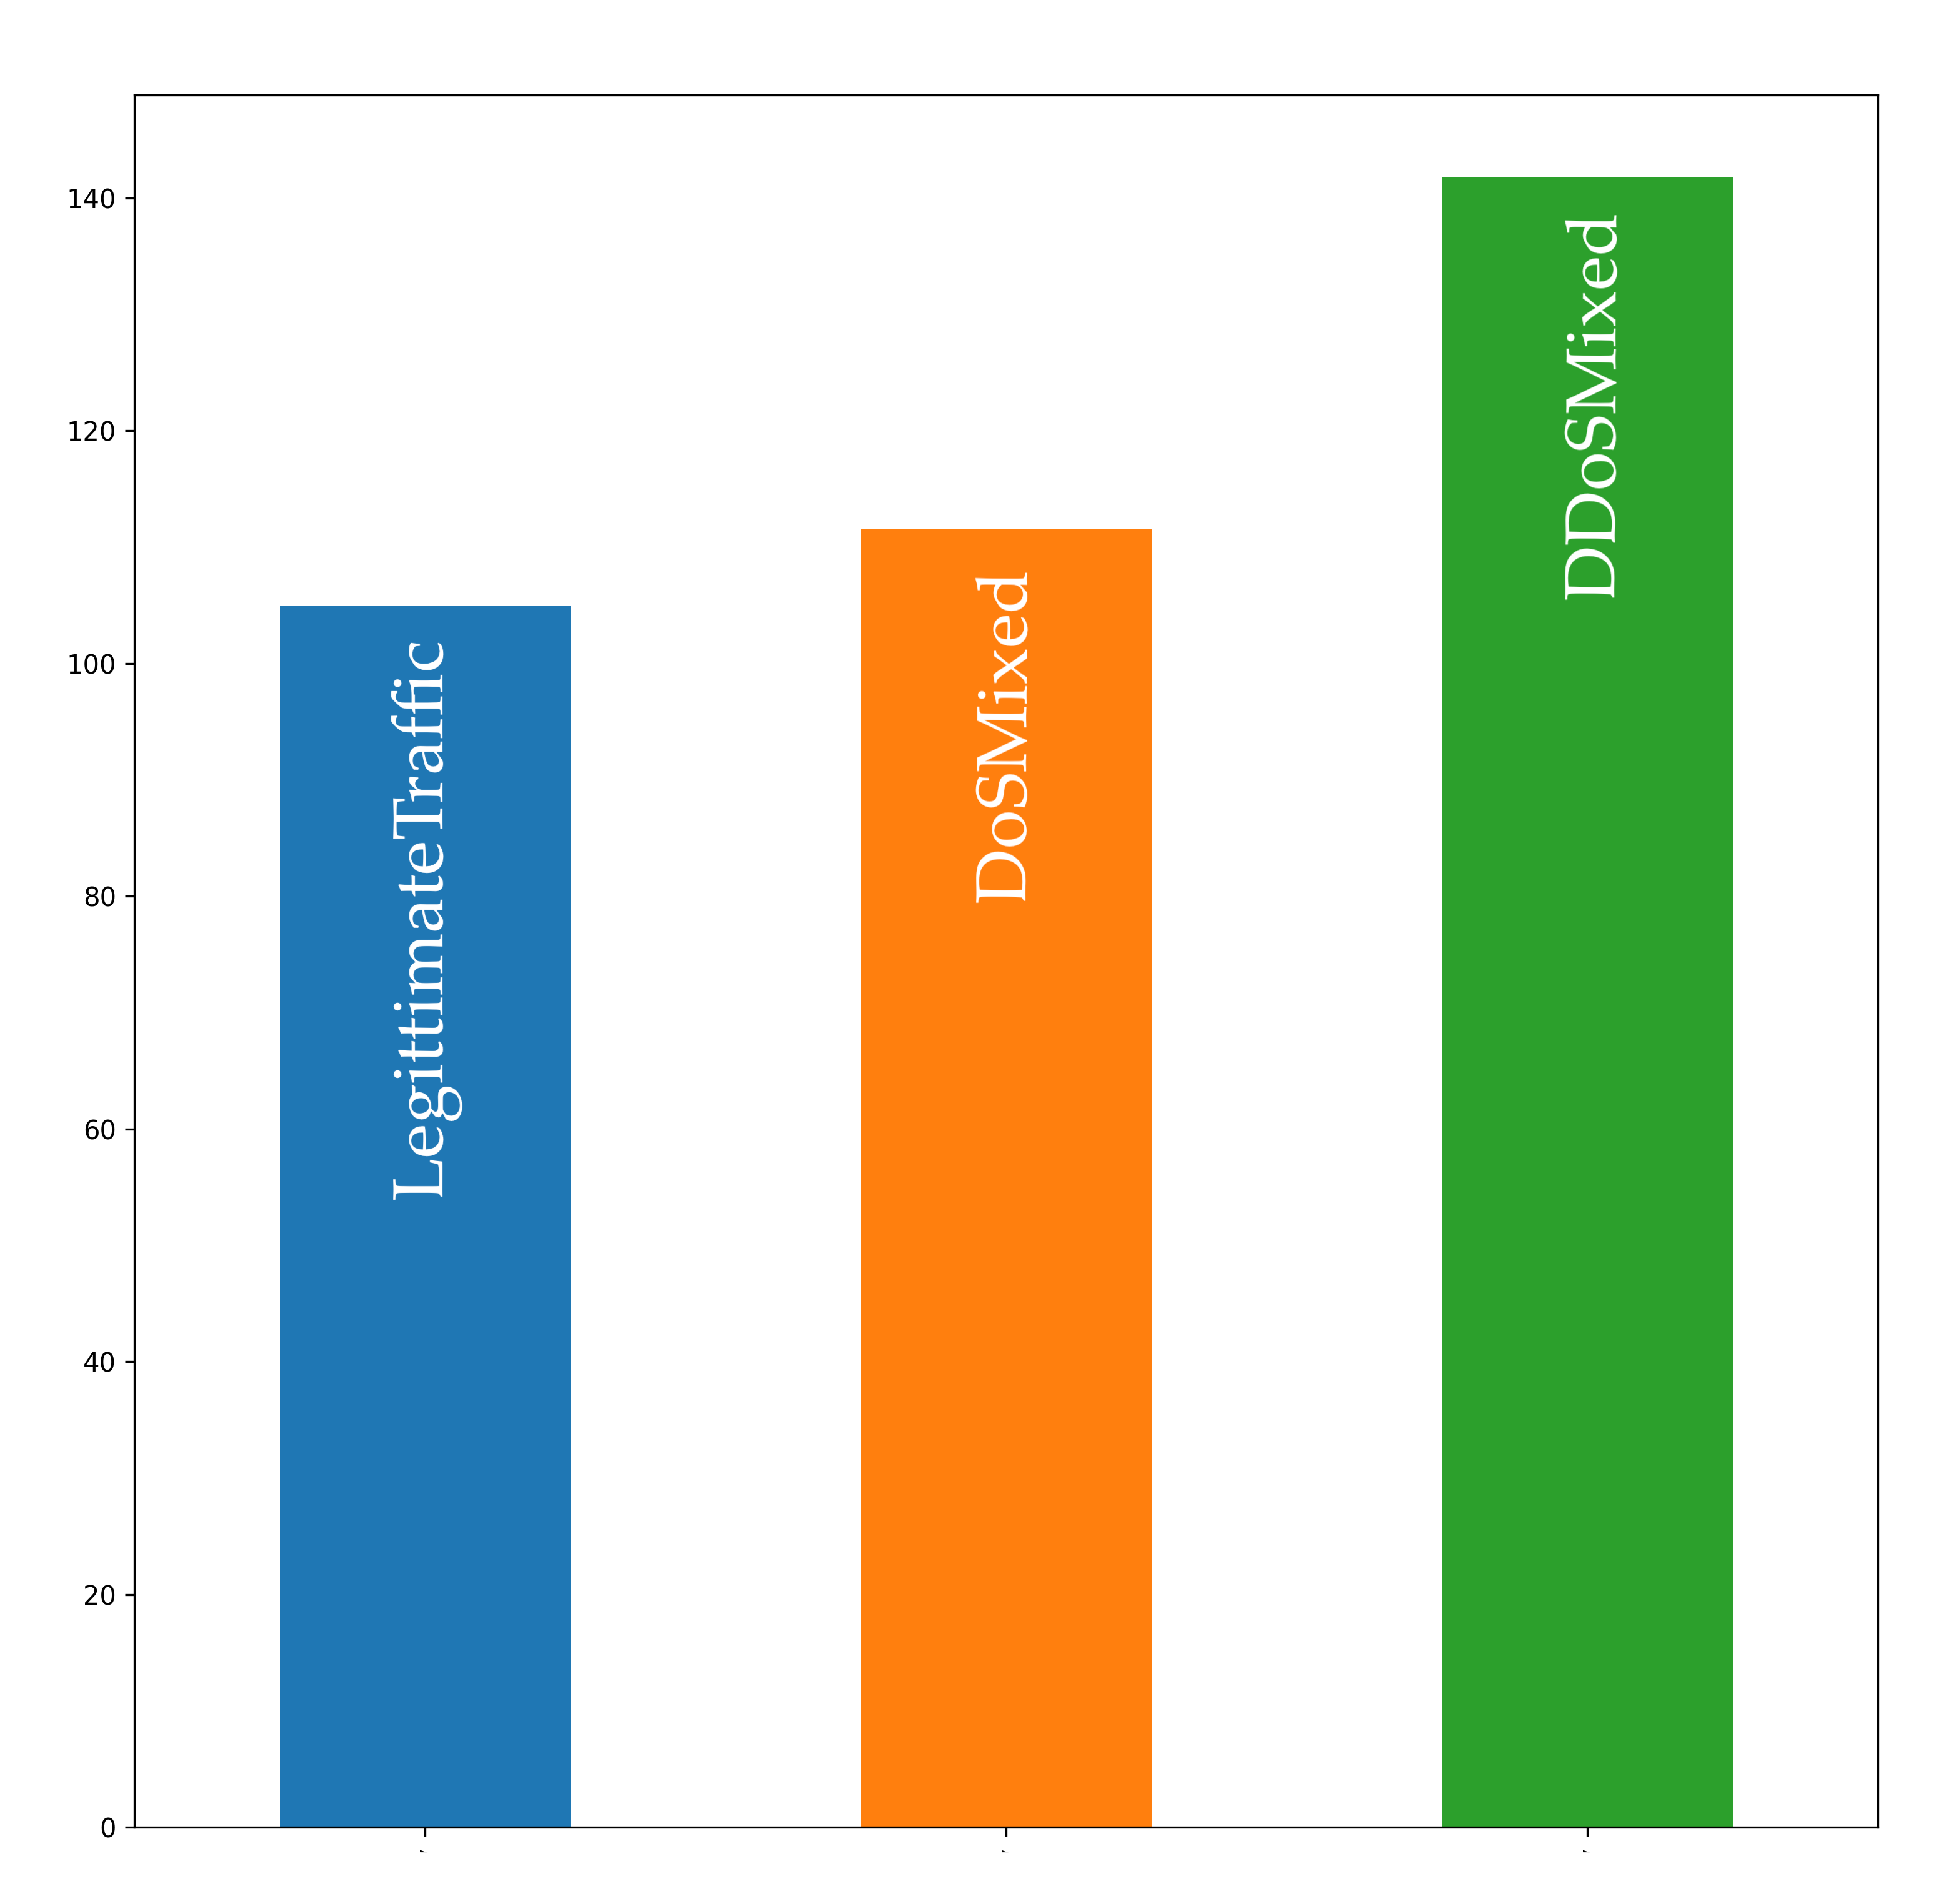
\includegraphics[scale=0.49]{imgs/analysis_stat.png}
%	\caption{Performance Analysis} 
%	\label{fig:analysis_stats}
%\end{figure}
In \textbf{Tab. \ref{tab:dataset_info}} we show a summary of the dimension of the datasets we have used in our analysis. Both the \textit{LegitimateTraffic} and \textit{DoSMixed} datasets were completed in approximately 1 minute and 40 seconds. \textit{DDosMixed} was completed in 2 minutes and 17 seconds, but it's not a noticeable increment, considering the fact that it's way bigger. This justifies the parallel approach we have used with \textbf{Pig Latin}.

\begin{table}[!htbp]
\centering
\begin{tabular}{|l|l|c|}
\hline
\textbf{Dataset} & \textbf{Description}                              & \textbf{Size} \\ \hline
LegitimateTraffic         & Traffic log in normal conditions. & 316 KB        \\ 
DoSMixed        & Traffic log during a DoS attack.                   & 89 MB       \\ 
DDoSMixed        & Traffic log during a DDoS attack. & 612 MB        \\ \hline
\end{tabular}
\caption{Datasets Info}
\label{tab:dataset_info}
\end{table}

\section{Conclusions}
\label{sec:colc}
We were inspired by \cite{detection_by_path_analaysis} and \cite{ddos_forensics} for the creation of our tool, we tried to find and follow a different approach for the analysis of DoS and DDoS attacks, proposed in the cited papers, and we decide to implement and use as mathematical models quantile range outliers, standard deviation and mean. Thanks to this approach we were able to bind big data power and python in order to manipulate and show analysis results.  

Focusing on the results over our generated datasets we conclude that the precision of our tool is high in \textit{UDP flood} attacks detection, but in order to evaluate the reliability of our tool we created a testbed to recreate real conditions and record exchanged traffic. The result are quiet good, our tool recognise attacker securely involved in the DoS or DDoS genesis but as side effect it may recognise some false positive user, these may be recognised easily using standard deviation and mean or by watching its reported data in order to evaluate manually if these candidates may be or not be in the attack. High precision is also achieved by not take into consideration IP address spoofing, which is a technique that give the possibility to an attacker to create Internet Protocol (IP) packets with a false source IP address, for the purpose of impersonating another computing system. In this work, we only consider the non-address spoofing flooding attack as assumed in \cite{ddos_forensics}. 

Tests over different kind of datasets will help the reliability evaluation of our tool by analyse real attack \textit{log} files, with the attackers labeled or highlighted, but these kind of datasets are difficult to retrive. 
Possible improvements may be done by try to implement new mathematical model which uses data prediction like \cite{detection_by_path_analaysis} and implement \textit{Pig-latin} script, similar to our, in order to detect other attacks like \textit{SYN ack flood} attack which is very common like \textit{UDP flood}. 
\newpage
\begin{thebibliography}{9}
\bibitem{ddos_forensics} 
Rana Khattak, Shehar Bano, Shujaat Hussain, Zahid Anwar. 
\\\textit{DOFUR: DDoS Forensics Using mapReduce}. Frontiers of Information Technology, 2011.

\bibitem{wireshrk_pcap}
Wireshark Wiki, Development. Last access \textit{May 15 2019}.
\\\url{https://wiki.wireshark.org/Development/LibpcapFileFormat}

\bibitem{detection_by_path_analaysis}
Theerasak Thapngam, Shui Yu, Wanlei Zhou, S. Kami Makki.
\\\textit{Distributed Denial of Service (DDoS) detection by traffic pattern analysis}.
Springer Science, 2012.

\bibitem{ddos_forensics}
Yinghua Guo, Ivan Lee.
\\\textit{Forensic analysis of DoS attack traffic in MANET}. 
Fourth International Conference on Network and System Security, 2010.

\end{thebibliography}
\end{document}